\documentclass[oneside]{scrbook} %KOMA-Script book
\usepackage[italian]{babel}
%Per i commenti
\usepackage{comment}
%Per l'interlinea
\usepackage{setspace}
%Codifica caratteri
\usepackage[utf8]{inputenc}
\usepackage{xspace}
\usepackage{eurosym}
%Fonts Scientifici
\usepackage{amsfonts}
\usepackage{amsmath}
\usepackage{amssymb}
\usepackage{textcomp}
%Pacchetto grafici
\usepackage{tikz}
\usepackage{pgfplots}
\pgfplotsset{/pgf/number format/use comma,compat=newest}
\usepackage{picture}
\usepackage{graphicx}
%Impostazioni tabelle avanzate e colorate
\usepackage{multicol}
\usepackage{multirow}
\usepackage{soul}
\usepackage{ulem}
\usepackage{booktabs}
%\usepackage{subfig}
\usepackage{subfigure}
\usepackage{array}
\usepackage{color}
\usepackage{colortbl}
%Pacchetto per gli pseudocodici
\usepackage{algpseudocode}
%\usepackage{listings}
\usepackage{listings,xcolor,courier,bookmark}
\usepackage{listingsutf8}
%Impostazioni tabelle avanzate
\usepackage{multicol}
\usepackage{multirow}
\usepackage{rotating}
\definecolor{darkblue}{named}{blue}
\definecolor{darkred}{named}{red}
\definecolor{grau}{named}{gray}
%Per i margini
\usepackage{chngpage}
\sloppy

\graphicspath{{Immagini/}}

\let\Righttorque\relax

\lstset{
	captionpos=b,
	commentstyle=\color[rgb]{0.133,0.545,0.133},
	keywordstyle=\color{darkblue},
	stringstyle=\color{purple},
	extendedchars=true,
	basicstyle=\small\ttfamily,
	showstringspaces=false,
	tabsize=2,
	numbers=left,
	numberstyle=\tiny,
	breakautoindent  = true,
	breakindent      = 2em,
	breaklines       = true,
	postbreak        = ,
	prebreak         = \raisebox{-.8ex}[0ex][0ex]{\Righttorque},
	showspaces=false,
	showtabs=false,
	showstringspaces=false,
	language=C++,
	frame=single,
	morecomment=[s]{°°}
}

\renewcommand*{\lstlistingname}{Codice}
\renewcommand*{\lstlistlistingname}{Elenco dei codici}

\usepackage{fancyhdr}
\pagestyle{fancy}
\renewcommand{\chaptermark}[1]{\markboth{\MakeUppercase{\thechapter.\ #1}}{}}
\fancypagestyle{plain} %stile delle pagine anche a quella iniziale del capitolo

\fancyhead{}
\fancyfoot{}

\fancyhead[R]{\bfseries \nouppercase{\leftmark}}
\fancyhead[L]{
	\includegraphics*[scale=0.8]{logo_dieti2.png}
}
\fancyfoot[R]{\thepage}
\fancyfoot[L]{Tesina di Impianti di Elaborazione}
\renewcommand{\headrulewidth}{0.4pt}
\renewcommand{\footrulewidth}{0.4pt}

\date{}
\cfoot{}
\usepackage{eso-pic,graphicx}

%Per sottosezioni
\setcounter{secnumdepth}{4}
\setcounter{tocdepth}{4}

\begin{document}

	% Per evitare che i collegamenti nell'indice abbiano i riquadri rossi
	\hypersetup {linkbordercolor=white}

	\AddToShipoutPicture{\AtPageCenter{\makebox(0,0){
\includegraphics{logo.png}}}}
	\frontmatter
	\pagenumbering{Roman}

	\begin{titlepage}
		\centering
		%{\Huge \textsc{Università degli Studi di Napoli ``Federico II''}}

		%\vspace*{\stretch{2.5}}

		%
\includegraphics[width=1\linewidth]{logo_federico_II.png}

		
\includegraphics[width=1\linewidth]{logo_dieti2.png}

		\vspace*{2cm}

		{\Huge \textsl{Tesina di\\IMPIANTI DI ELABORAZIONE}\par}

		\vspace*{2cm}

		{\huge \text{Prof. Domenico Cotroneo}}

		\vspace*{5cm}

		{\LARGE \textit{Andrea Scognamiglio - Matr. M63/598\\Cristian Tommasino - Matr. M63/615}}

		\vspace*{2.5cm}

		{\Large \textsc{A.A. 2017/2018}}
	\end{titlepage}

	\setcounter{page}{1}

	\newpage
	\tableofcontents

	\newpage
	\mainmatter

	% !TEX root = ./main.tex
% !TEX encoding = UTF-8 Unicode
% !TEX program = pdflatex
% !TeX spellcheck = it_IT

\graphicspath{{Immagini/},{Immagini/ffda/}}

\chapter{Field Failure Data Analysis}
La \textbf{FFDA} è effettuata sui dati relativi ad un sistema in
esercizio(\textit{on Field}), al fine di scoprire i possibili fallimenti.\\
L'approccio utilizzato nella FFDA prevede di monitorare il sistema in esecuzione,
misurando parametri di dependability e prelevando tutte le possibili informazioni
sul fallimenti rilevati.\\
Un fallimento è una deviazione del comportamento del sistema dal suo corretto e
specifico funzionamento.\\
La metodologia FFDA è basata su tre fasi fondamentali:
\begin{itemize}
  \item \textbf{Data Logging \& Collection} - consiste nella definizione di cosa
  collezionare e come farlo;
  \item \textbf{Data Filtering \& Manipulation} - consiste nella manipolazione ù
  dei dati collezionati, utilizzando \textit{filtering} e \textit{coalescence};
  \item \textbf{Data Logging \& Collection} - consiste nell'esecuzione di un'analisi
  statistica su dati precedentemente manipolati, per calcolarne misure quantitative
  e identificarne possibili trends.\\
\end{itemize}

\section{Traccia}
Dati i due file di log \textit{MercuryErrorLog} e \textit{BGLErrorLog},
preventivamente filtrati per ottenere solo eventi di fallimento, si vuole:
\begin{itemize}
  \item determinare la finestra di coalescenza;
  \item raggruppare tutte le entry appartenenti alle stesse finestre di
  coalescenza(tuple);
  \item ricavare la \textit{CDF} del \textbf{TTF}(Time-To-Failure) e della
  \textbf{Reliability Empirica};
  \item fitting della CDF della reliability empirica provando tutti i modelli
  studiati (\textit{Esponenziale}, \textit{Weibull} ed \textit{Iperesponenziale});
  \item utilizzare il test di \textit{Kolmogorov-Smirnov} per controllare che il
  modello ipotizzato fitti adeguatamente i dati.\\
\end{itemize}

\clearpage

\section{Mercury}
Il sistema Mercury consiste di nodi IBM.\\
Il cluster ha un'architettura a 3 livelli(nodi \textit{login}, \textit{computation}
e \textit{storage}) ed un solo nodo di management
(\textit{tg-master}).\\
Il log è formato dai seguenti campi:
\begin{itemize}
  \item \textbf{Timestamp};
  \item \textbf{Nodo Origine};
  \item \textbf{Categoria Errore}:
  \begin{itemize}
    \item DEV, PRO, MEM, NET, IO, OTH;
  \end{itemize}
  \item \textbf{Messaggio}.
\end{itemize}

\subsection{Finestra di Coalescenza - CWIN}
La finestra di coalescence, definita in secondi, definisce un intervallo temporale
in cui cadono tutti gli eventi che vi appartengono.\\
Lo script \textbf{tupleCount\_func\_CWINpy.sh}(riportato in figura \ref{coalescence_window_mercury}), con input i file \textit{MercuryErrorLog.txt}
e \textit{tentative-CWIN.txt}, è stato utilizzato per calcolare il numero di tuple al
variare della dimensione della finestra di coalescenza.\\

\begin{figure}[!htbp]
  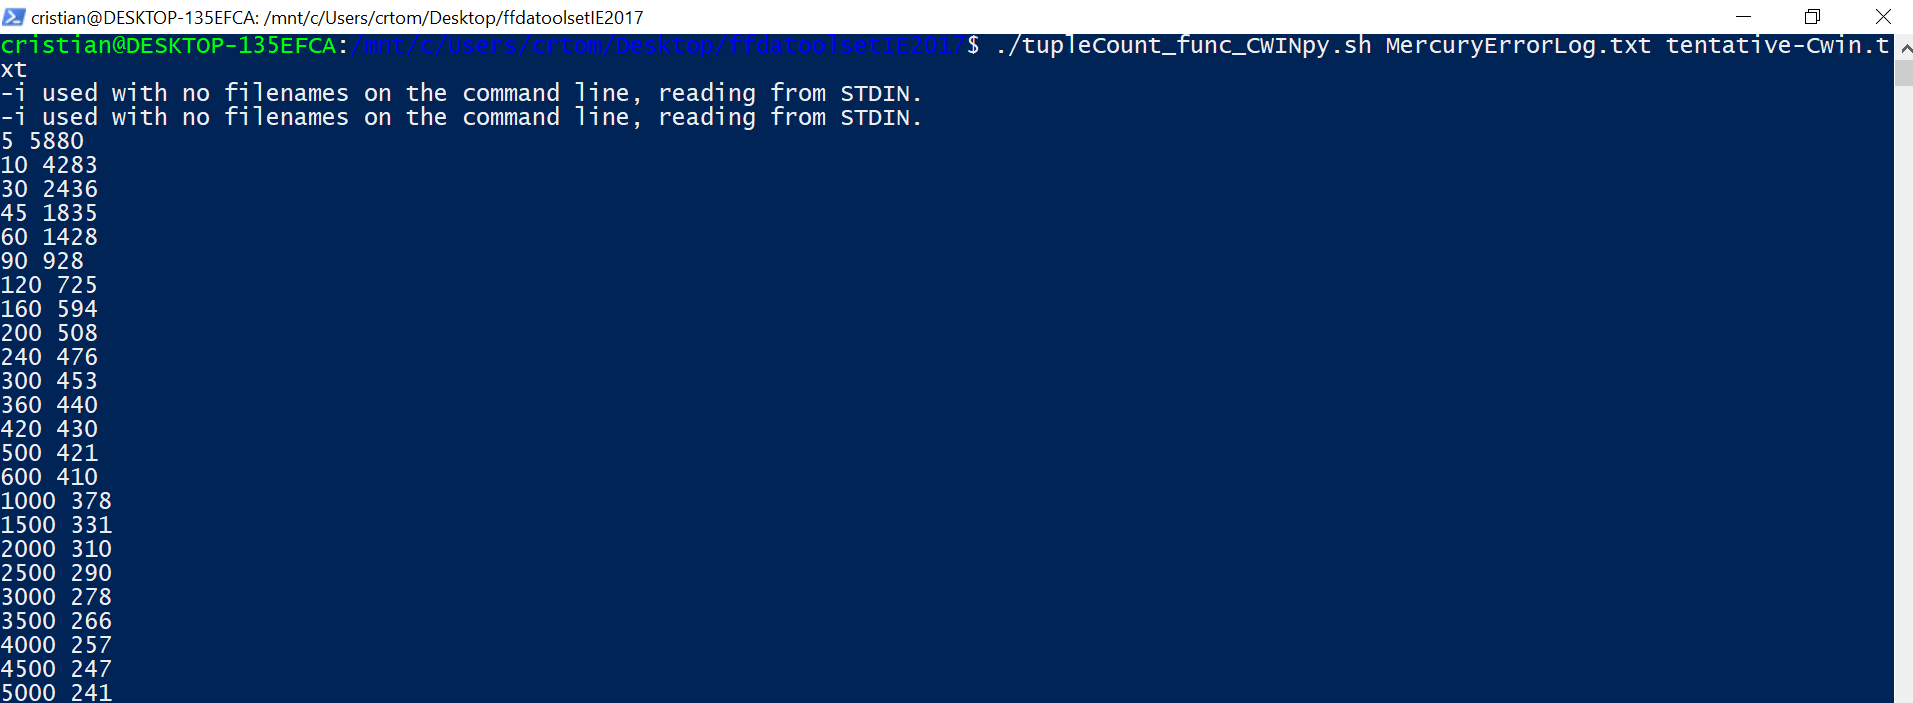
\includegraphics[width=1\linewidth,keepaspectratio]{coalescence_window_mercury}
  \caption{Script conteggio tuple al variare della finestra di coalescenza}
  \label{coalescence_window_mercury}
\end{figure}

\clearpage

L'output di tale script, plottato in matlab e presente in figura \ref{plot_coalescence_window_mercury},
è infine utilizzato per determinare un singolo valore di CWIN, ottenuto
considerando il punto successivo al ginocchio(knee) della curva.\\

\begin{figure}[!htbp]
  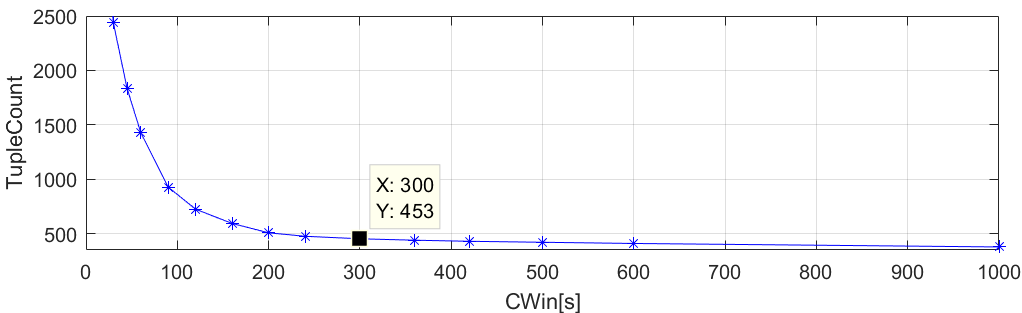
\includegraphics[width=1\linewidth,keepaspectratio]{plot_coalescence_window_mercury}
  \caption{Plot finestre di coalescenza}
  \label{plot_coalescence_window_mercury}
\end{figure}

%%ANDREA è ARRIVATO QUI!!!


\end{document}
